% Chapter 5
\chapter{Advertisement Low fidelity prototype} % Main chapter title

\label{Chapter5} % For referencing the chapter elsewhere, use \ref{Chapter1} 

\section{Introduction}
During the last focus-group discussions and all gathered data from attraction attention study and interviews, the first paper prototype of interactive advertisement was decided to be created. This document describes the advertisement application requirements, lists all functionalities along with its use cases and defines the target group that this application is going to be made for. 

Paper prototype for Bauhaus-Walk [14] shows two different interactions (body and mobile) and tries to give an overall general picture of how the advertisement would look like after development, but to test this paper prototype, this document purposes a test design for complete evaluation of all important functionalities.

\newpage
\section{Requirement gathering}

The bellow mentions Bauhaus-Walk advertisement?s all functional and non-functional requirements and what system requirement would be required at the time of development.

\subsection{Functional Requirements}

\begin{enumerate}
\item	Detect multi User.
\item	Assign a character to the user. 
\item	Assign a task to the user.
\item	Respond to each user interaction.
\item	Show advertisement text.
\item	End the interaction.
\end{enumerate}


\subsection{Non-functional Requirements}

\begin{enumerate}
\item	Performance \\
This is a very important requirement that should be wisely done. Response time should be very fast in both gesture and mobile interaction so the user could see the reaction quickly on the screen. 

\item	Scalability \\
The interaction is scalable for multi-users at the same time for body interaction and mobile interaction.

\item	Availability \\
Kinect camera should be functional during the experiment for people detection, Access point should be running so that it could provide network access to users.

\item	Usability \\
The advertisement interaction both mobile and body should meet all criteria of usability.
\end{enumerate}

\section{Personas}
The bellow personas are made based on focus group findings that most of people taking tour are elder people, which builds up our primary type of persona and secondary type persona would be young age girl as described bellow.




\hilight{put the persona table here}



\section{Use case diagrams}



\hilight{put good use case diagrams }


\section{Goal}
The goal of this evaluation is to find possible issues as listed bellow with interactive advertisement. 

\begin{enumerate}
\item   Confusing events
\item   Unclear events or interactions.
\item   Misconception of a function.
\item   Task confusion.
\item   Understandability of advertisement goal and contents.
\end{enumerate}


\subsection{Hypothesis}
Hypothesis are divided for each individual interactions like mobile and body.

\subsubsection{Body Interaction}

\begin{itemize}

\item H1: Users understand and react to the Call-to-Action approach.
\item H2: Users recognizes the character assigned to them.
\item H3: Users understands the tasks assigned to them.
\item H4: Users can explore locations by moving their body in physical space.
\item H5: Application raises alerts to specific user actions.
\item H6: Application motivates participants to continue playing.
\end{itemize}

\subsection{Mobile Interaction}

\begin{itemize}
\item H1: Users understand the Access Information shown on the board.
\item H2: Users open the controller website by scanning QR-Code.
\item H3: Webpage application produces alerts with in correct user input.
\item H4: Users rotate the mobile phone to start game.
\item H5: Users understand the task.
\item H6: Users can navigate the character by moving the face in mobile.
\item H7: Screen application produces alerts for incorrect location.
\end{itemize}

\section{Design study}
Bauhaus-Walk interactive advertisement consist of two elements, first is the screen that the users see the reaction and advertisement content, and the second is the means of interaction which are body and mobile, to design the test first of all the paper prototype should be capable to show both of these elements to be applicable to the real scenario later.  

Actual advertisement screen paper prototype would be made along with its all interactive objects and as well as mobile paper prototype for user interaction would also be printed we would not need any paper prototype for gesture interaction. I as an experimenter would simulate all user actions on the display even actions like movement of silhouette or character face


\begin{figure}[H]
    \centering
    \subfloat[]{{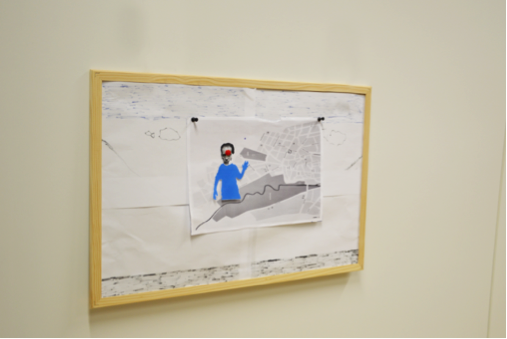
\includegraphics[width=6cm,height=4cm]{Figures/5/paper_board} }}%
    \hfill
    \subfloat[]{{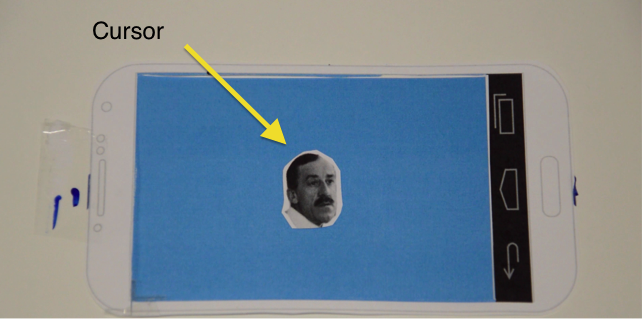
\includegraphics[width=6cm,height=4cm]{Figures/5/mobile_paper} }}%
    \caption{A: Screen paper prototype. B: Mobile paper prototype. }%
    \label{fig:paper_prototype}%
\end{figure}



\subsection{Subjects}
Five participants were invited to experience with the paper prototype.
The participants were from different background, like Media Art, Media architecture and computer science.

\subsection{Location}
Participants were invited in Digital Bauhaus Lab ground floor, where the environment was prepared for the paper prototype interaction.


\subsection{Procedures}
The test subjects will be given basically one task by the interactive advertisement screen and by user body movement their location on the paper screen would be changed and checked for possible interactive object so that the content could be changed and for mobile interaction the subjects will be instructed to think-aloud while interacting with mobile interface so that examiner be able to change content on paper screen.

\begin{figure}[H]
    \centering
    \subfloat[]{{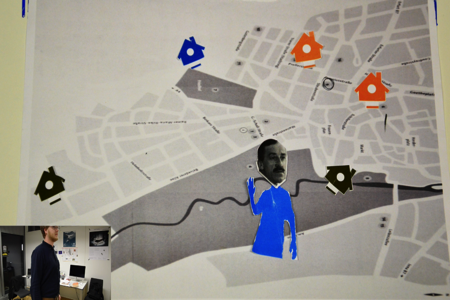
\includegraphics[width=6cm,height=4cm]{Figures/5/body_interaction} }}%
    \hfill
    \subfloat[]{{\includegraphics[width=6cm,height=4cm]{Figures/5/mobile_interactions} }}%
    \caption{A: Body interaction.  B: Mobile Interaction. }%
    \label{fig:Interactive_prototype}%
\end{figure}



\section{Data gathering}
The process of data gathering was as bellow, the methods are designed in a way to fully answer the research questions and the defined hypothesis.


\begin{enumerate}
\item Video Recording \\
Each participant was video recorded for both body and mobile interactions for later observation and analyzing purpose. 

\item Direct observation \\
Participants were observed during the interaction and also asked about what they thought at that moment while interacting. When participants could not perform a task then they were asked exploratory questions on how would they do the task naturally.

\item Think aloud \\
Participants were asked to read their mind while interacting with the prototypes. This helped to understand what they thought about a specific interaction at that moment. 

\item Interviews \\
After both paper prototype interactions were finished, a brief interview was taken to further learn about the interactions they did and get other user comments and feedbacks for the prototypes.
\end{enumerate}


\section{Findings}
The important part for analyzing the data is shaped based on the defined hypothesis at the beginning; the bellow procedure was followed to best answer our open questions and to be able to evaluate both paper prototypes. For interview codings see Appendix \ref{AppendixC}


\subsection{Usability issues}


\subsection{Body Interactions usability}

\begin{enumerate}
\item Confusions 

\begin{enumerate}
\item  Participant was confused of how should to walk, because it felt that there is not enough space. 
\item  User thought that if he/she moves to the location names or the icons, someone would guide her.
\item  User was confused on the new character photo labeled on the top of his silhouette; he thought that the new character is trying to interact with his silhouette. ``\emph{Is it like people approaching you and say hi and hello, and then ask me if I can visit his places}''
\item  He did not know his places (the character’s places).
\item  Could not understood the word move or walk, he taught that it is not applicable at the moment.
\item  Raise one hand to see if the blue reacts or not.
\item  Did not recognize the person.
\item  Did not understand the task.
\item  Did not understand what is the blue person.
\item  Asked question about who is the face, he did not know it.

\end{enumerate}

\item Frustrations
\begin{enumerate}
\item  Entering IP address.
\item  When the wrong house was explored, and she said ``\emph{(Ohh No)}''.
\item  Waiting for the houses to load on the screen.
\end{enumerate}

\item Mistakes
\begin{enumerate}
\item  Entered to the wrong location.
\item  Did not know how to navigate to the places. Even he was told that the silhouette is his body.
\item  Navigating the silhouette was a problem for her; she wanted to go on top of the map in the screen but physically moved back. And after seeing the reaction she corrected herself.
\end{enumerate}

\item Comments
\begin{enumerate}

\item   There should be very clear instruction in the application on what to do, what it is about and how to do it.
\item   I did not understand the person; maybe do not use it anymore.


\end{enumerate}
\end{enumerate}


\subsection{Mobile usability}
The bellow chart lists all the possible issues with mobile interaction.

\begin{enumerate}

\item Confusions
\begin{enumerate}
\item  The idea of the application was not clear for her because she taught that the mobile application could be used when she goes out in the city. But later she found out that the screen and mobile are both of them used at a place.
\item  Navigation was a big confusion for him; he was touching the character on the mobile screen.
\item  The turning phone as shown in arrow, since she could not turn the phone.
\item  Did not understood what happened after the interaction was over. She did not read the texts or she did not understand why those were about.
\item  The face in the mobile.
\end{enumerate}

\item Frustrations
\begin{enumerate}
\item  Visiting to all locations to finish the interaction.
\item  Not enough things when visiting to a location.
\item  She felt frustrated when visiting the wrong location and find the right location.
\item  He had to re-login because he accidently pressed cancel button.
\item  Visited to the wrong location.
\item  Waiting for the houses to load on the screen.
\end{enumerate}

\item Mistakes
\begin{enumerate}
\item  Did not understand to scan QR code.
\item  Took longer time to use the phone prototype. 
\item  Did not understand to rotate the mobile. As the instructions were shown on the phone.
\item  Took longer time to navigate the person on the screen.
\item  She tried to continue without putting any name in the form.
\item  Did not understand how to turn the phone, she touched the arrow on the screen many times. But nothing happened. Later she knew to turn the phone, but did not do it because she thought that the paper prototype should not be moved from its place.
\item  Could not navigate the person on the screen.
\item  Entered the wrong IP address, but then changed his mind and scanned the QR code.
\item  Accidently pressed cancel.
\end{enumerate}

\item Comments
\begin{enumerate}
\item  There is no enough information about the locations; it would be good to show a short description of the place.
\item  There could be like choices like when the opening time is for these locations.
\item  How far are they from my current location, the distance?
\item  View the transport possibilities to the selected locations.
\item  It would be good to have more information about the locations.
\item  And I would like to see the entire map on the phone too.
\item  I like to see some more information in my phone.
\item  There should be more guides when I use the phone, like there should be like Samsung, when you turn it on for the first time, it shows how to use what or it should have a finger picture to swipe on the face.
\end{enumerate}

\end{enumerate}

This chart was created to list all the possible, mistakes, misunderstandings and confusions for each of the interactions carried by participants, these lists were categorized under usability problem. This error chart was made during video observations, flow of the tasks were observed and also the words they used during interaction from which confusion, frustration and misunderstandings events were recorded. 

Looking through all the usability problem chart of each participant the bellow single chart is being created, each category is separately listed with the possible problems.


\subsection{Hypothesis decisions}

The hypothesis those were defined in the design study, from which some of them are accepted and rejected based on the above findings. 

\subsubsection{Body Interaction}
\begin{itemize}
\item H1: Users understand and react to the Call-to-Action approach.\\ 
\textbf{[Accepted]}\\
All of the participants understood call-to-action and reacted to it quickly as soon they read it.

\item H2: Users recognizes the character assigned to them.\\ 
\textbf{[Rejected]}\\
All the participants did not understand the character which was assigned to them, This happens when the participants do not have background to the related history that should know the character, It would be better to use someone who is very famous and is known to most of the population and different cultures, using very specific character is a bad idea. Users gets confused. At one occasion even an architect student who must know that face, but unfortunately did not recognized him. 

\item H3: Users understands the tasks assigned to them.  \\ 
\textbf{[Rejected]}\\
Most users did not understand the task in the sense of the defined character, but they did understand that they should walk and explore locations.

\item H4: Users can explore locations by moving their body in physical space. \\ 
\textbf{[Accepted]}\\
As soon they understand that the silhouette is them and projected on the screen, then they did the task by moving them selves physically, except one participant who did not understand until the observer gave him hint to move his self physically in right or left.

\item H5: Application raises alerts to specific user actions.   \\ 
\textbf{[Rejected]}\\
The application did not raised error for user?s specific interactions like if the user was out of the screen or very close to the screen. Most of the participants raised their hand up, or turned around, there was no alerts for the participants.

\item H6: Application motivates participants to continue playing. \\ 
\textbf{[Rejected]}\\
When the users explored the first location, they were excited and tried to see the other places, but all the locations action was predictable by the participants and nothing new was happening, participants expected more from their interactions to be more excited to play the whole game. They did finish the game because they were told so.

\end{itemize}


\subsubsection {Mobile Interaction}
\begin{itemize}
\item H1: Users understand the Access Information shown on the board. \\ 
\textbf{[Accepted]}\\
The participants were not shown the phone prototype at first, they were only shown the display and were asked to react based on the messages or what ever the users comprehend, after reading the Access information they asked for the phone prototype and then the phone prototype was shown to them to interact.

\item H2: Users open the controller website by scanning QR-Code. \\ 
\textbf{[Accepted]}\\
Four of the participants understood the use of QR-code and from which two of them scanned it and other two typed the IP address, and one participant did not understood the use of QR-code.

\item H3: Webpage application produces alerts with in correct user input.\\ 
\textbf{[Rejected]}\\
The webpage did not produce error at many occasions while filling the form like, what happens when cancel button is pressed, or when the game finishes the application does not alert user to replay or leave webpage.

\item H4: Users rotate the mobile phone to start game.\\ 
\textbf{[Rejected]}\\
Only two of the participants rotated the phone but the rest of the participants tapped on the icon and tried to rotate the icon in the screen instead rotating the whole phone.

\item H5: Users understand the task.\\ 
\textbf{[Rejected]}\\
This happened because all of the participants did not recognized the face and did not know where are his locations.

\item H6: Users can navigate the character by moving the face in mobile.\\ 
\textbf{[Rejected]}\\
Four of the participants touched and tapped the face shown on the mobile phone many times, they expected that something will happen after they touch the character like a dropdown list would appear to edit it, but one of the users drag it and saw the reaction on the screen.

\item H7: Screen application produces alerts for incorrect location.\\ 
\textbf{[Accepted]}\\
The incorrect locations that were explored by the participants were given an alert message.
\end{itemize}



\newpage
\section{Conclusions}

Evaluation of low-fidelity prototype of advertisement was very helpful to understand possible design problems and interactions that could have been a headache if had identified at high-fidelity version. 

First, the body interaction was easily understood by most of the participants, this type of interaction is more natural and can be done by any kind of participant without having any technical expertise. Two most important interactions in this technique was the call-to-action which approached participants to come near to the screen and other was to explore the locations using their body position in physical space. This low-fidelity usability testing suggests bringing changes for the next high-fidelity version of the advertisement. The changes would be to remove the character assigning for individuals, improving alert messages for different user actions, improving task description and integrating features to increase interest rate for participants to be engaged with the advertisement.

Second, participants also appreciated the mobile interaction, but they were not so convinced for the usage because of many issues like logging in web application first, then navigating the face character. There was no clear instructions for how to navigate the character, and what will happen if there are many participants playing at the same time, where all of the participant would have the same face and they would get confused that which one is being controlled by their controller and lastly, it was unclear that what happens in web application when the interaction is over. This usability testing helped us to identify the mention usability problems and would bring changes for the new high fidelity version that would solve the current issues.

Third, The advertisement text, which was shown at the end of interaction, did not brought user?s attention, it would be better to make a short video for the next prototype that could bring users attention to see the advertisement. After the video advertisement gets over the attraction phase starts again.

Finally, all hypotheses that were accepted or reject will be taken in to account from which new decisions for the high fidelity version will be taken, this version will overcome all the issues discovered until this stage. Participant?s recommendations and feedbacks have also much value and would be considered in the development phase.








